% Options for packages loaded elsewhere
\PassOptionsToPackage{unicode}{hyperref}
\PassOptionsToPackage{hyphens}{url}
%
\documentclass[
]{article}
\usepackage{amsmath,amssymb}
\usepackage{lmodern}
\usepackage{iftex}
\ifPDFTeX
  \usepackage[T1]{fontenc}
  \usepackage[utf8]{inputenc}
  \usepackage{textcomp} % provide euro and other symbols
\else % if luatex or xetex
  \usepackage{unicode-math}
  \defaultfontfeatures{Scale=MatchLowercase}
  \defaultfontfeatures[\rmfamily]{Ligatures=TeX,Scale=1}
\fi
% Use upquote if available, for straight quotes in verbatim environments
\IfFileExists{upquote.sty}{\usepackage{upquote}}{}
\IfFileExists{microtype.sty}{% use microtype if available
  \usepackage[]{microtype}
  \UseMicrotypeSet[protrusion]{basicmath} % disable protrusion for tt fonts
}{}
\makeatletter
\@ifundefined{KOMAClassName}{% if non-KOMA class
  \IfFileExists{parskip.sty}{%
    \usepackage{parskip}
  }{% else
    \setlength{\parindent}{0pt}
    \setlength{\parskip}{6pt plus 2pt minus 1pt}}
}{% if KOMA class
  \KOMAoptions{parskip=half}}
\makeatother
\usepackage{xcolor}
\usepackage[margin=1in]{geometry}
\usepackage{graphicx}
\makeatletter
\def\maxwidth{\ifdim\Gin@nat@width>\linewidth\linewidth\else\Gin@nat@width\fi}
\def\maxheight{\ifdim\Gin@nat@height>\textheight\textheight\else\Gin@nat@height\fi}
\makeatother
% Scale images if necessary, so that they will not overflow the page
% margins by default, and it is still possible to overwrite the defaults
% using explicit options in \includegraphics[width, height, ...]{}
\setkeys{Gin}{width=\maxwidth,height=\maxheight,keepaspectratio}
% Set default figure placement to htbp
\makeatletter
\def\fps@figure{htbp}
\makeatother
\setlength{\emergencystretch}{3em} % prevent overfull lines
\providecommand{\tightlist}{%
  \setlength{\itemsep}{0pt}\setlength{\parskip}{0pt}}
\setcounter{secnumdepth}{-\maxdimen} % remove section numbering
\ifLuaTeX
  \usepackage{selnolig}  % disable illegal ligatures
\fi
\IfFileExists{bookmark.sty}{\usepackage{bookmark}}{\usepackage{hyperref}}
\IfFileExists{xurl.sty}{\usepackage{xurl}}{} % add URL line breaks if available
\urlstyle{same} % disable monospaced font for URLs
\hypersetup{
  hidelinks,
  pdfcreator={LaTeX via pandoc}}

\author{}
\date{\vspace{-2.5em}}

\begin{document}

\href{https://github.com/CamposecoKevin/CV/blob/main/CV-KC/KevinCamposeco_English.pdf}{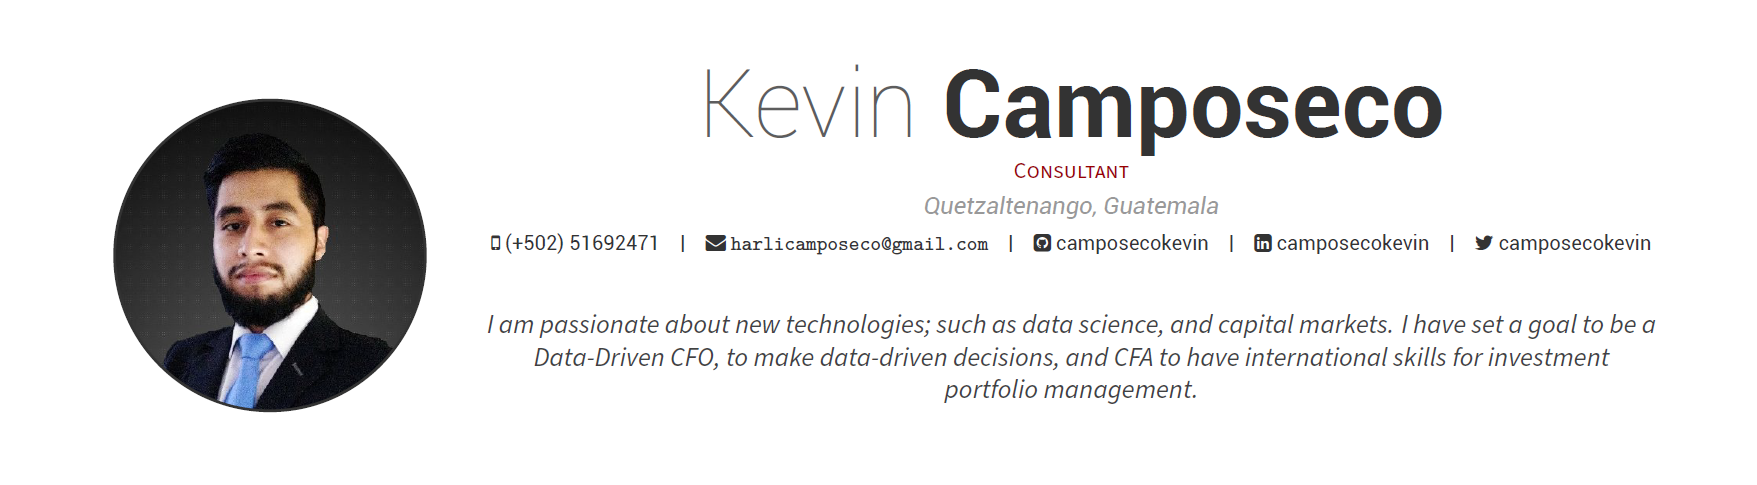
\includegraphics{https://github.com/CamposecoKevin/CV/blob/main/CV-KC/img/coverpage_Kevin.png}}
\# My RESUMÉ \#\#\#
\href{https://github.com/CamposecoKevin/CV/blob/main/CV-KC/KevinCamposeco_English.pdf}{English
version CV} \#\#\#
\href{https://github.com/CamposecoKevin/CV/blob/main/CV-KC/KevinCamposeco_Español.pdf}{Spanish
version CV}

\hypertarget{what}{%
\subsection{What}\label{what}}

This CV is created using the \textbf{\texttt{R}} Package
\href{https://github.com/mitchelloharawild/vitae}{\texttt{vitae}}

\begin{center}\rule{0.5\linewidth}{0.5pt}\end{center}

\begin{quote}
\emph{\textbf{Curriculum Vitae}}

A brief summary of my resume to apply for a position.

\begin{center}\rule{0.5\linewidth}{0.5pt}\end{center}
\end{quote}

\hypertarget{why}{%
\subsection{Why}\label{why}}

Task automation is a necessity, especially when looking to make
data-driven decisions. And that's what I did with a my CV, I needed a CV
that I could easily update, and that was easily accessible when I needed
it.

\hypertarget{how}{%
\subsection{How}\label{how}}

This document was compiled in the \textbf{Rmarkdown} environment, using
the pandoc library.

And in thanks to Bryan Jenks, I leave his cv repository
\url{https://github.com/tallguyjenks/CV} for you to review, it was a
great help in the creation of my own cv.

\end{document}
